%!TEX root = /Users/stefan/projects/papers/paper.4/paper.tex
\begin{figure*}[!t]
\begin{center}
\subfloat[node real]
{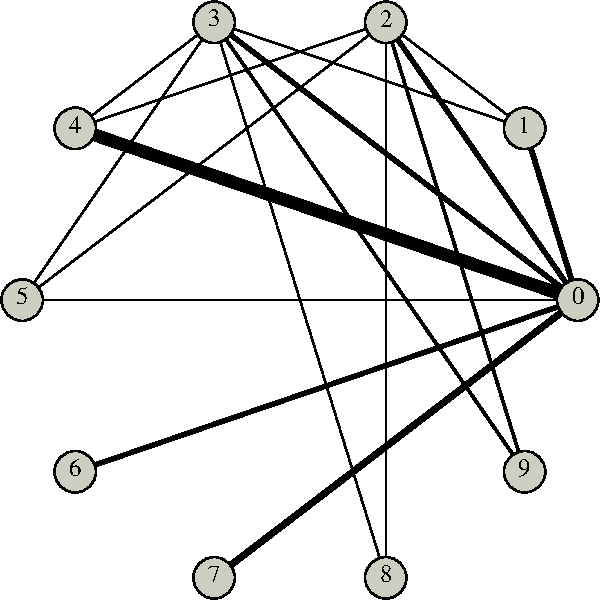
\includegraphics[width=1.335in]{flow_topology_trace}\label{fig:flow-topology-trace}}
\subfloat[node uniform]
{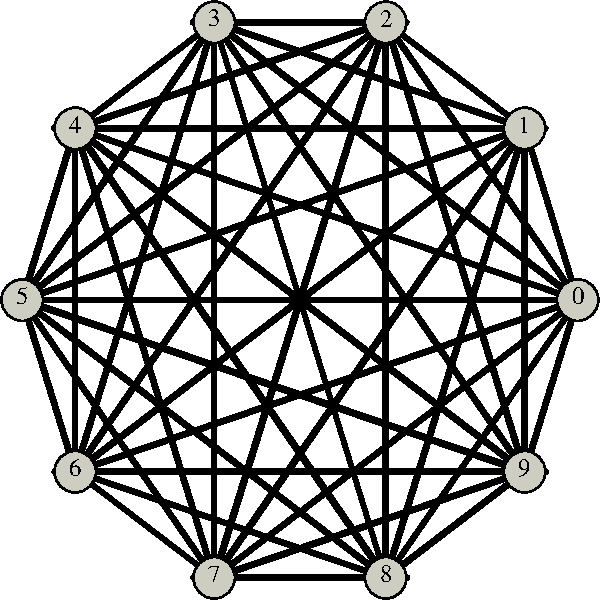
\includegraphics[width=1.335in]{flow_topology_uniform}\label{fig:flow-topology-uniform}}
\subfloat[flow real]
{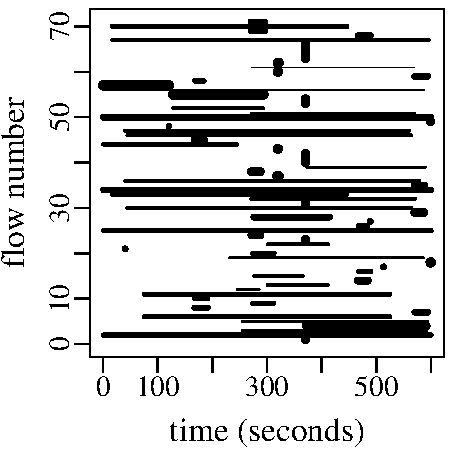
\includegraphics[width=1.335in]{flow_behavior_trace}\label{fig:flow-behavior-trace}}
\subfloat[flow uniform]
{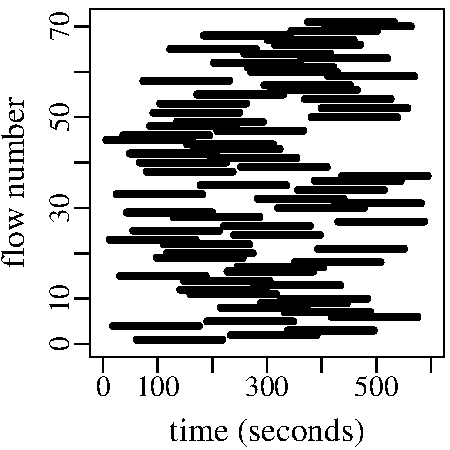
\includegraphics[width=1.335in]{flow_behavior_uniform}\label{fig:flow-behavior-uniform}}
\subfloat[packet]
{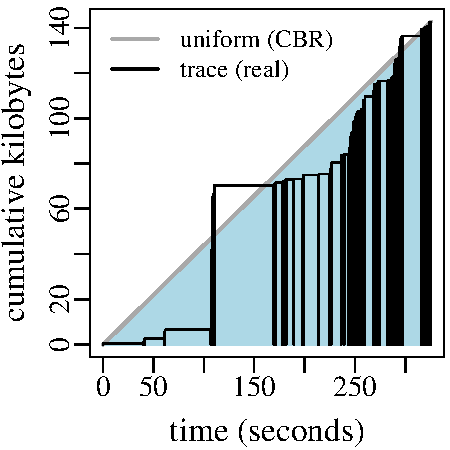
\includegraphics[width=1.335in]{flow_packet_behavior}\label{fig:packet-behavior}}
\caption{Examples illustrating real versus uniform behaviors at the node, flow and packet levels. Figures \ref{fig:flow-topology-trace} and \ref{fig:flow-topology-uniform} show example node behaviors. The width of each line is proportional to the logarithm of the number of flows between the nodes (zero is the Internet gateway). Uniform and trace flow behavior examples are plotted in Figures \ref{fig:flow-behavior-trace} and \ref{fig:flow-behavior-uniform}. The time axis indicates when flows start and end; the width of each flow line is proportional to the logarithm of its data rate. Figure \ref{fig:packet-behavior} compares uniform (i.e. \caps{CBR}) packet behavior with the trace of an actual flow. In the uniform model, the cumulative data sent increases smoothly over time, whereas in the actual packet trace, the transmissions are variable both in size and in inter-packet interval, leading to a ``lumpy'' cumulative data plot.}
\label{fig:trace-vs-uniform}
\end{center}
\vspace{-1.25em}
\end{figure*}
